\documentclass{kththesis}


%Taken from ID1354
\usepackage[utf8]{inputenc}
\usepackage[english]{babel}
\usepackage{graphicx}
\usepackage{lastpage}
\usepackage{pgf}
\usepackage{wrapfig}
\usepackage{fancyvrb}
\usepackage{fancyhdr}
\pagestyle{fancy}
\usepackage{dingbat}

\usepackage[autostyle]{csquotes}
\usepackage[
    backend=biber,
    style=ieee,
    sortlocale=de_DE,
    natbib=true,
    url=true,
    doi=true,
    eprint=false
]{biblatex}
\addbibresource{references.bib}

\usepackage[]{hyperref}
\hypersetup{
    colorlinks=true,
}

% List of abbreviations
\usepackage{glossaries}
\makeglossaries

\title{This is the English title}
\alttitle{Detta är den svenska översättningen av titeln}
\author{Jacob Kimblad}
\email{jacobki@kth.se}
\supervisor{Matthias Becker}
\examiner{Zhonghai Lu}
\programme{Master's Programme in Embedded Systems}
\school{School of Electrical Engineering and Computer Science}
\date{\today}


\begin{document}

%Term definitions
\newacronym{os}{OS}{Operating System}
\newacronym{cpu}{CPU}{Central Processing Unit}
\newacronym{lcu}{LCU}{Central Processing Unit}
\newacronym{aer}{AER}{Acquisition Execution Restitution}
\newacronym{cots}{COTS}{Commerical off the Shelf}
\newacronym{edf}{EDF}{Earliest Deadline First}
\newacronym{rms}{RMS}{Rate-Monotonic Scheduling}
\newacronym{lcm}{LCM}{Least Common Multiple}

% Frontmatter includes the title page, abstracts and table-of-contents
\frontmatter

\titlepage

\begin{abstract} 

    English abstract goes here.

\end{abstract}


\begin{otherlanguage}{Swedish} 
    
    \begin{abstract}

    \end{abstract} 

\end{otherlanguage}

% List of Acronyms
\printglossary[title={Acronyms}]

% Table of contents
%\tableofcontents

% Mainmatter is where the actual contents of the thesis goes
\mainmatter


\chapter{Introduction} 
temp
Embedded systems in the automotive sector are required to go through a lot of analysis and testing
before being deemed safe for use in traffic. With the rise of autonomous vehicles these systems are
becoming more complex as an effect of more computing needed being done.  This has also put
requirements on the hardware to become faster and faster, thus the industry is turning to the use of
multi-core and many-core platforms. These type of platforms present more unpredictability than
single-core platforms which requires new methods of analysis and deterministic execution of these
systems. 


\section{Background} 

Timing analysis is an important part of real-time systems. However, multi-core platforms often
implement complicated memory hierarchies that make timing analysis a lot harder. One way to tackle
this is to schedule the access to shared memory in cooperation with computational tasks. This can
improve analysis and is employed by industrial domains already where the execution of tasks can be
divided up into three distinct parts, read-execute-write.


\section{Problem}

An analysis method for resource contention in multi-core real-time systems have been proposed in
paper [1]. This analysis method is however not 1 Template for project proposal 2018-12-12 customised
for the read-execute-write execution model that is adapted both within the avionics domain and
automotive domain.


\section{Purpose}

The purpose is to expand existing analysis methods by adding to the source code and/or produce a
model of the read-execute-write task model that is available as input for these formal analysis
methods.


\section{Goal}



\subsection{Benefits, Ethics and Sustainability}

\section{Methodology / Methods}

\section{Delimitations}

\section{Outline}


%We use the \emph{biblatex} package to handle our references.  We therefore use the command
%\texttt{parencite} to get a reference in parenthesis, like this \parencite{heisenberg2015}.  It is
%also possible to include the author as part of the sentence using \texttt{textcite}, like talking
%about the work of \textcite{einstein2016}.

\chapter{<Theoretic Background> Use a self-explaining title}



\section{The Task Model} \label{sec:the_task_model}

A periodic task, denoted as $\tau_i$, is a unit of work that is executed periodically on a processor
alongside other tasks over and over again. In embedded systems a task is usually completed in some
amount of time known as its \textbf{computation time}, denoted as $C_i$. Once a task has finished
executing it will usually wait for some amount of time before it is ready to execute again, this is
known as the tasks \textbf{period}, denoted by $T_i$. The earliest time where a task is ready to
start execution within a new period is called the \textbf{arrival time} of the task and is denoted $
a_i $. Note that the arrival time is equal to the beginning of a specific period for the task.

The \acrshort{lcm} of the periods for all the tasks in a task set is known as the task set's
\textbf{hyper-period} and is an important concept in scheduling tasks which is further discussed
in section \ref{sec:scheduling}. The hyper-period is defined as $H = \acrshort{lcm}(P_i)$ for $i =
1, 2, ..., n$. Each task is also required to finish execution before a set amount of time starting
from each new period belonging to the specific task, this is known as the task's \textbf{relative
deadline} denoted as $D_i$. For an \acrshort{os} to decide in what order the tasks should execute
when more than one is available at the same time they are each assigned a \textbf{priority}, denoted
by $P_i$, by a scheduler which is further discussed in section \ref{sec:scheduling}. A task can thus
be introduced by defining its characteristics as $\tau_i = (T_i, C_i)$. It is then also possible to
define a task set as $ \Gamma = \{\tau_1, \tau_2, \tau_3, ..., \tau_n\} $.

Following the above definitions state can be can ascribed to tasks depending on their status in the
system at a specific time instance. A task is in the \textit{ready} state when it still needs time
to complete its execution before its deadline but is not yet allowed access to the processor. Once a
task is moved out of the ready state and is executing on the \acrshort{cpu} it is said that the task
is \textit{running}. The task can also be moved back to the ready state from running state before
execution is finished by being \textbf{preempted} by the scheduler. If a task requires access to
some shared resource that is not currently available, thus halting execution, the task is said to be
\textit{waiting}. Once the shared resource is available again the task is moved back into the ready
state. The three different states and their transitioning are depicted in figure
\ref{fig:ready-running-blocked-model}.

\begin{figure}

    \centering

    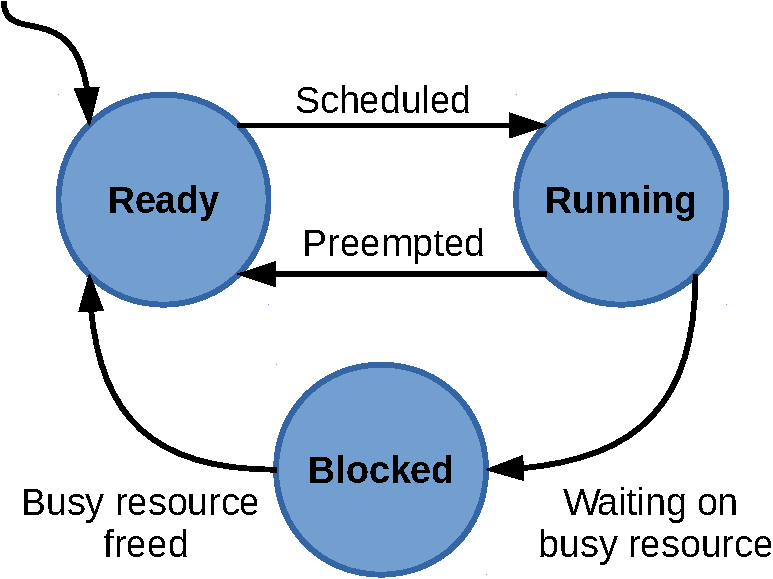
\includegraphics[width=0.7\linewidth]{images/ready-running-blocked-model.pdf}

    \caption{The three states a task may be in.}

    \label{fig:ready-running-blocked-model}

\end{figure}

% TODO: talk about aperiodic and sporadic tasks as well? 
\section{Scheduling} \label{sec:scheduling}

Although computers give away the illusion of being able to deal with many things simultaneously this
is actually not the case. Computers are limited to how much parallel computing they are able to do
by the hardware, specifically the amount of cores within the \acrshort{cpu}. A computer with, for
example, a single core \acrshort{cpu} is only able to execute one task at a time. For a computer
with a single core to deal with more than a single task at the same time requires switching ongoing
tasks in and out of the core during runtime. For the \acrshort{os} to switch tasks quickly in and
out of the core it needs to schedule the tasks according to some order. This is where the priority
of tasks come in handy, by scheduling tasks and switching them in and out of the processor very
quickly depending on their priority the \acrshort{os} is able to perform more than one task seemingly in
parallel than what is actually allowed for by hardware. The rest of this section up until section
\ref{subsec:multiprocessor-scheduling} is only concerned with the scheduling of single core
processors.

% TODO Maybe add other measurements of how good schedulers are, least-slack time etc.
The order in which tasks are executed is determined by the scheduler which in of itself is a special
type of task executed by the \acrshort{os}. The scheduler is invoked by specific events happening in
the system. It could for example be that a task is finished executing or that it has begun waiting
on some resource that is not yet available. As not all scheduling algorithms were created equal they
vary in how good of a task they do when scheduling the same task sets. Because of this some
measurements must be introduced in order to have a fair comparison of how well they work. The
processor utilization factor, denoted as $ U $, is such a measurement introduced to show to what
percentage a specific task set would keep the processor busy if scheduled optimally. The utilization
can be calculated as such $ U = \sum_{i=1}^n \frac{e_i}{P_i} $.

For embedded systems there exists a set of well known scheduling algorithms such as \acrshort{edf}
and \acrshort{rms}. Imagining a single-core \acrshort{cpu} the algorithm \acrshort{rms} works by
setting the priority of each task equals to its period. This means that the task with the lowest
period is given the highest priority and always scheduled first once it is in the ready state. Since
periods of tasks never changes during execution, the priorities of the individual tasks will never
change either, thus \acrshort{rms} is said to be a \textbf{static-priority scheduler}. If a
scheduler instead changes the priorities of the task during execution it is a
\textbf{dynamic-priority scheduler}. 

Instead of setting priorities according to the periods, \acrshort{edf} works by setting the
priorities according to how close a task is to its deadline. This means that the task closest to
exceeding its deadline will always be executing first on the processor. If some task $ \tau_a $ is
executing with a deadline further away in time than another task $ \tau_b $, that was just released,
then $ \tau_a $ will get preempted and the newly released $ \tau_b $ will be allowed to execute
instead. This behaviour makes \acrshort{edf} a \textbf{preemptive scheduling algorithm}, the
opposite of which is a \textbf{non-preemptive scheduling algorithm} which lets each task finish
before scheduling the next highest priority task.

An example of how \acrshort{rms} would schedule a task set can be seen in figure
\ref{fig:rate-monotonic-scheduling}. A special point of interest is at time 4 when $T_3$ is
executing from earlier as $T_1$ is released. As $T_1$ has a lower period than $T_3$ it also has
a higher priority. The scheduler preempts $T_3$ and instead lets $T_1$ execute before $T_3$ is
allowed to resume execution of $j_3$ at time 5.

\begin{figure}

    \centering

    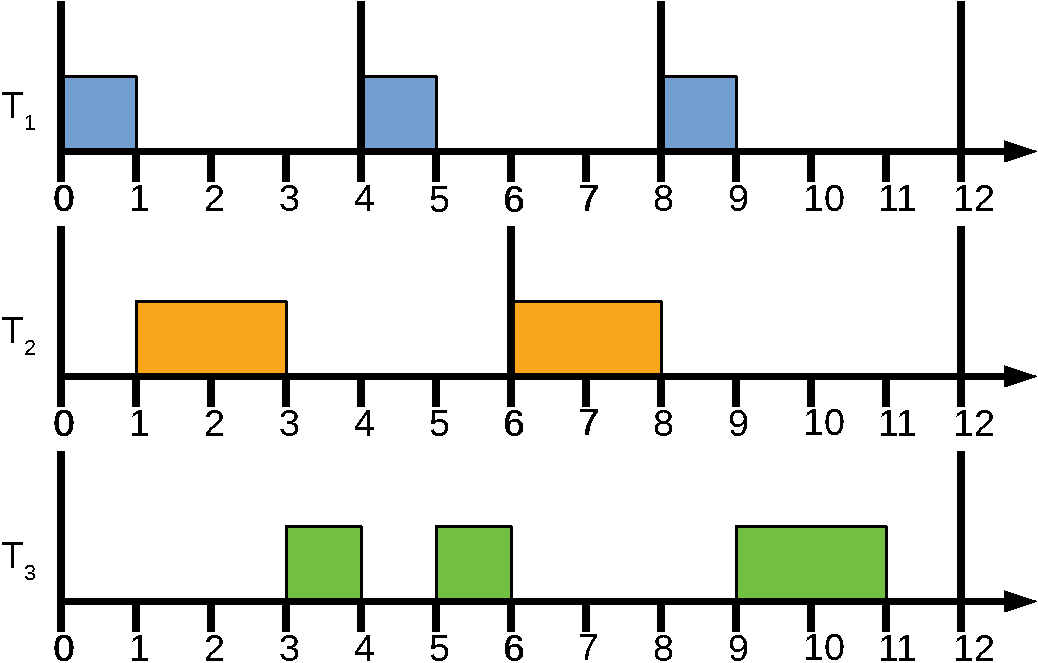
\includegraphics[width=0.8\linewidth]{images/rate-monotonic-scheduling.pdf}

    \caption{Example of rate monotonic scheduling for three tasks where $T_1=(4, 4, 1)$, $T_2=(6, 6,
    2)$, $T_3=(12, 12, 4)$.}

    \label{fig:rate-monotonic-scheduling}

\end{figure}

\subsection{Multiprocessor scheduling} \label{subsec:multiprocessor-scheduling}

When considering multiprocessors life for schedulers become a little harder. The additional
questions that have to be answered is  

% TODO Talk about global scheduling

\section{Schedulability testing}

When developing new scheduling methods it is important to put the schedules that they produce under
analysis as to show that they are feasible. It is especially important when the schedules are used
in hard real-time systems like those found in the avionics and the automotive sector were missed
deadlines could mean fatal outcome. \acrshort{rms} for example can be analysed mathematically and
has been proven to be able to schedule any set of tasks that utilizes the processor to a degree less
than $\ln (2)\%$ and more precisely be able to schedule any set of tasks that satisfies $U =
\sum_{i=1}^n \frac{e_i}{P_i} \le n(2^{\frac{1}{n}}-1)$.  This means that \acrshort{rms} might not be
able to find a feasible schedule even if one exists. This makes \acrshort{rms}
\textbf{non-optimal}. In contrast \acrshort{edf} has been proven to always find a feasible schedule
for preemptive single-core systems if one exists, making it \textbf{optimal} in those circumstances.

% TODO explain optimal vs. non-optimal scheduling algorithms
% TODO example of the formula that is a sufficient schedulability test for 
% TODO introduce the concept of WCET and BCET as well as release-time jitter in this section and
% explain how it helps to make analysis of multicore systems much harder

\section{The AER Execution Model}

The \acrshort{aer} execution model was first proposed in \parencite{durrieu_predictable_2014} to
improve performance and predictability while using \acrshort{cots} multi-core processors with
distributed memory in the avionics industry. Since the bottleneck for these types of systems often
is the access to shared memory \acrshort{aer} focuses on making it more deterministic and easier to
analyse. This is done by dividing up the tasks that run within an \acrshort{os} into three distinct
parts.

%TODO Do we first explain what a task is, that it runs on a single core within a multi-processor and
%that for this industry it often is non-greedy when it is non-preemptive. Do we go into detail of
%the task model (running, ready and executing), this is probably good to cover in the global
%scheduling part.

The paper \parencite{maia_closer_2016} takes a closer look i

\chapter{<Engineering-related content, Methodologies and Methods> Use a self-explaining title}


\chapter{<The work> Use a self-explaining title}


\chapter{<Result> Use a self-explaining title}


\chapter{<Conclusions> Use a self-explaining title}


% Print the bibliography (and make it appear in the table of contents)
\printbibliography[heading=bibintoc] 

% Start the appendix section
\appendix

% Appendix A
\chapter{Unnecessary Appended Material}


\end{document}
